\section{Результаты расчётов}

\subsection{Вычислительная среда}

Расчёты выполнены 9 ноября 2026 года на IBM Polus.
Планировщик LSF выделил два вычислительных узла в исключительное пользование на время серии.
Каждый узел содержит два процессора POWER8NVL, по десять физических ядер в каждом.
Одно ядро поддерживает восемь аппаратных потоков, поэтому операционная система видит 160 логических процессоров на узел.
Аппаратные потоки одного ядра разделяют его вычислительные ресурсы.

Все четыре версии собраны GCC 7.3.1 из Advance Toolchain 11.0 с параметрами \code{-std=c++17 -O3 -DNDEBUG -mcpu=power8}.
Использованы Spectrum MPI 10.1.0 и библиотека OpenMP \code{libgomp} из той же поставки GCC.
Порог остановки основных расчётов равен $\delta=10^{-8}$.

Последовательная версия привязана к одному логическому процессору.
В конфигурациях OpenMP до 16 потоков каждый поток занимает отдельное физическое ядро.
Конфигурация с 32 потоками использует 16 физических ядер, по два аппаратных потока на ядро (SMT2).
Ядра выбираются поочерёдно из двух процессорных сокетов.
Динамическое изменение числа потоков отключено.

В MPI каждому процессу выделено отдельное ядро, а в гибридной версии каждому потоку процесса выделено своё ядро.
MPI с 32 процессами размещается по 16 процессов на двух узлах.
Гибридная конфигурация $4\times8$ использует по два процесса с восемью потоками на каждом узле.
Остальные конфигурации выполняются на одном узле.
Число процессов и потоков, имена узлов и назначенные логические процессоры проверены для каждого запуска.

\subsection{Протокол измерений}

Выполнены оба набора конфигураций из задания: основной набор на малых сетках и полный набор приложения на сетках $400\times600$ и $800\times1200$~\cite{assignment}.
С учётом последовательных базовых расчётов серия содержит 37 конфигураций.
Перед измерениями каждая из них запускалась один раз для прогрева.
Для малых сеток проведено семь измерительных повторов, для крупных три.
Порядок конфигураций перемешивался с начальным значением генератора $14$.
Всего получено 155 измерений времени; прогревы и отдельный запуск для сохранения поля решения в статистику не входят.

Время $T$ измеряется внутри программы и включает выделение и инициализацию рабочих векторов, итерации метода сопряжённых градиентов, MPI-обмены и редукции.
Подготовка геометрии, запуск процессов, финальная проверка невязки и запись CSV выполняются вне измеряемого участка.
Для MPI и гибридной версии берётся максимум времени по процессам.
В таблицах приведены медиана и диапазон от минимального до максимального времени; все повторы сохранены, включая выбросы.

Ускорение вычисляется относительно отдельной последовательной программы на той же сетке:
\begin{equation}
    S(P,T_{\rm th})=\frac{T_{\rm seq}}{T_{P,T_{\rm th}}}.
    \label{eq:speedup}
\end{equation}
Здесь $P$ обозначает число процессов, $T_{\rm th}$ число потоков в процессе, а времена в правой части являются медианами повторов.
Значение $S<1$ соответствует замедлению относительно последовательной версии.
На графиках отрезки разброса ограничены величинами $T_{\rm seq,min}/T_{\rm par,max}$ и $T_{\rm seq,max}/T_{\rm par,min}$.
Они показывают диапазон отношений наблюдавшихся времён и не являются доверительными интервалами.

\FloatBarrier
\subsection{Последовательное решение}

Число итераций растёт при сгущении сетки (табл.~\ref{tab:seq}).
На каждой сетке оно одинаково у всех четырёх реализаций.
Все основные запуски завершились по критерию~\eqref{eq:stop} без перезапуска метода.
Невязка вычислена после остановки по системе для поправки~\eqref{eq:shifted}.
Её норма увеличивается при сгущении сетки: выбранный критерий ограничивает изменение приближения между итерациями и не задаёт фиксированной нормы невязки.

\begin{table}[H]
    \PaperTableStyle
    \begin{threeparttable}
        \caption{Последовательные расчёты на Polus}
        \label{tab:seq}
        \begin{tabular*}{\linewidth}{@{\extracolsep{\fill}}rrrrr@{}}
            \toprule
            \textbf{Сетка} & \textbf{Итер.} & \textbf{$T$, с} & \textbf{Диапазон, с} & \textbf{$\normE{\vect r}$}\\
            \midrule
            \DataInput{sequential_rows}
            \bottomrule
        \end{tabular*}
        \begin{tablenotes}[flushleft]\PaperTableNotesStyle
            \item[] Семь повторов на малых сетках и три на крупных; $\vect r=\vect b-\mat A\vect w$. Приведена наибольшая норма невязки среди повторов.
        \end{tablenotes}
    \end{threeparttable}
\end{table}

Решение на сетке $800\times1200$ показано на рис.~\ref{fig:solution}.
Эта сетка содержит $962001$ узел, из них $958001$ внутренних неизвестных.
Внутри $D$ значения приближения лежат примерно от $-1.000$ до $3.195$.
На цветовой карте фиктивная область скрыта.
Сечение при $x=0$ показывает изменение решения внутри области относительно продолжения граничной функции $g$.
Функция $g$ используется в постановке штрафной задачи; точное решение исходной задачи неизвестно.

\begin{figure}[ht]
    \centering
    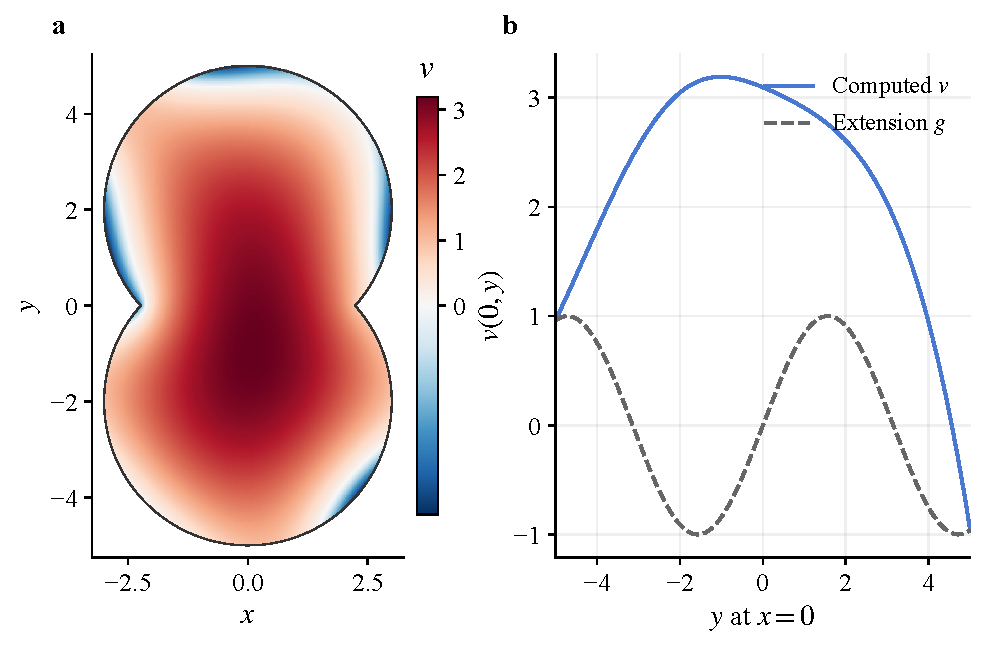
\includegraphics[width=\linewidth]{figures/solution.pdf}
    \caption{Решение на сетке $800\times1200$, полученное на Polus при $\varepsilon=h^2$ и $\delta=10^{-8}$: \textbf{a} значения $v$ внутри $D$; \textbf{b} сечение $v(0,y)$ и функция $g(0,y)=\sin y$. Последняя задаёт продолжение граничных данных, с которым сравнивается форма сечения.}
    \label{fig:solution}
\end{figure}

\FloatBarrier
\subsection{Проверка точности}

Для проверки численного метода решена вспомогательная задача с известным решением $v_*(x,y)=\sin(x+y)$.
В ней правая часть уравнения~\eqref{eq:penalty} заменена на $F_*(x,y)=2\sin(x+y)$ во всём прямоугольнике; коэффициент $Q$ и граничные условия сохранены.
Поскольку $-\Delta v_*=2v_*$ и $v_*-g=0$, эта функция точно удовлетворяет вспомогательной дифференциальной задаче при любом $\varepsilon$.
Проверяется ошибка
\begin{equation}
    E_h=\max_{1\leq i<M,\,1\leq j<N}|v_{ij}-v_*(x_i,y_j)|, \qquad p_h=\log_2\frac{E_{2h}}{E_h}.
\end{equation}
Величина $p_h$ оценивает наблюдаемый порядок уменьшения ошибки при двукратном сгущении сетки.

\begin{table}[H]
    \PaperTableStyle
    \begin{threeparttable}
        \caption{Проверка на известном решении}
        \label{tab:accuracy}
        \begin{tabular*}{\linewidth}{@{\extracolsep{\fill}}rrrr@{}}
            \toprule
            \textbf{Сетка} & \textbf{$h$} & \textbf{$E_h$} & \textbf{$p_h$}\\
            \midrule
            \DataInput{accuracy_rows}
            \bottomrule
        \end{tabular*}
        \begin{tablenotes}[flushleft]\PaperTableNotesStyle
            \item[] Проверка выполнена на Polus при $\delta=10^{-10}$. Порядок для первой строки не определяется.
        \end{tablenotes}
    \end{threeparttable}
\end{table}

Ошибки уменьшаются примерно в четыре раза при двукратном уменьшении шага.
График на рис.~\ref{fig:convergence} согласуется с зависимостью $E_h\sim h^2$ для выбранной гладкой тестовой функции.
Проверка подтверждает согласованность разностного оператора, граничных условий и решателя.
Порядок точности для исходной задачи с разрывной правой частью и приближённым условием на криволинейной границе отдельно не исследовался.

\begin{figure}[ht]
    \centering
    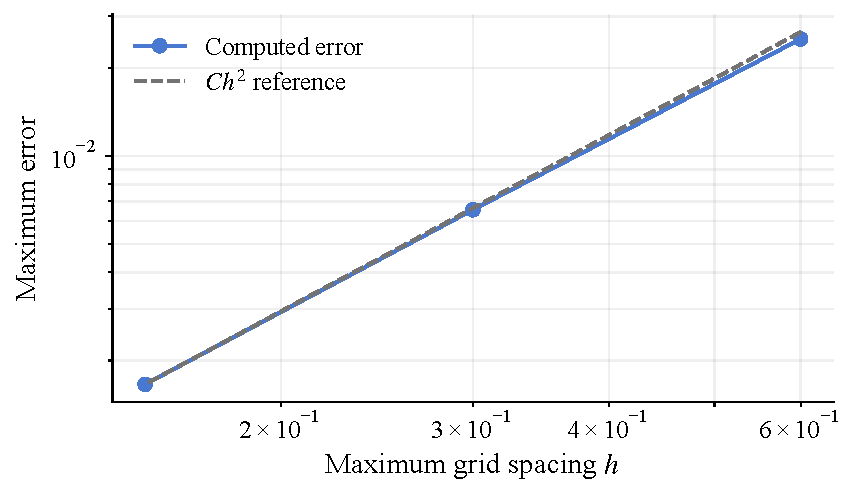
\includegraphics[width=0.82\linewidth]{figures/convergence.pdf}
    \caption{Максимальная ошибка для точного решения $v_* = \sin(x+y)$ на трёх сетках. Пунктирная линия пропорциональна $h^2$ и нормирована по ошибке на самой мелкой сетке. Обе оси логарифмические.}
    \label{fig:convergence}
\end{figure}

На сетке $6\times8$ результат сравнивался с независимым плотным решением системы методом исключения Гаусса.
В этой проверке площади ячеек получены численным интегрированием горизонтальных сечений.
При $\delta=10^{-10}$ максимальное различие составило $1.27\cdot10^{-7}$.
На сетках $23\times31$ и $80\times80$ решения последовательной и параллельных версий совпали с максимальным различием менее $8\cdot10^{-15}$ при том же пороге.
Первая сетка дополнительно проверяет неравномерное MPI-разбиение.

\FloatBarrier
\subsection{Малая сетка}

На сетке $80\times80$ все версии выполнили $193$ итерации для $6241$ неизвестного (табл.~\ref{tab:omp}, \ref{tab:mpi}, \ref{tab:hybrid}).
При сравнении используется медиана последовательного времени $16.420$ мс.

\begin{table}[H]
    \PaperTableStyle
    \begin{threeparttable}
        \caption{OpenMP на сетке $80\times80$}
        \label{tab:omp}
        \begin{tabular*}{\linewidth}{@{\extracolsep{\fill}}rrrrr@{}}
            \toprule
            \textbf{Потоки} & \textbf{Итерации} & \textbf{$T$, мс} & \textbf{Диапазон, мс} & \textbf{$S$}\\
            \midrule
            \DataInput{omp_rows}
            \bottomrule
        \end{tabular*}
        \begin{tablenotes}[flushleft]\PaperTableNotesStyle
            \item[] Семь повторов на одном узле. Каждый поток занимает отдельное физическое ядро.
        \end{tablenotes}
    \end{threeparttable}
\end{table}

\begin{table}[H]
    \PaperTableStyle
    \begin{threeparttable}
        \caption{MPI на сетке $80\times80$}
        \label{tab:mpi}
        \begin{tabular*}{\linewidth}{@{\extracolsep{\fill}}rrrrr@{}}
            \toprule
            \textbf{Процессы} & \textbf{Итерации} & \textbf{$T$, мс} & \textbf{Диапазон, мс} & \textbf{$S$}\\
            \midrule
            \DataInput{mpi_rows}
            \bottomrule
        \end{tabular*}
        \begin{tablenotes}[flushleft]\PaperTableNotesStyle
            \item[] Семь повторов; все процессы работают на одном узле и используют отдельные физические ядра.
        \end{tablenotes}
    \end{threeparttable}
\end{table}

\begin{table}[H]
    \PaperTableStyle
    \begin{threeparttable}
        \caption{MPI+OpenMP на сетке $80\times80$}
        \label{tab:hybrid}
        \begin{tabular*}{\linewidth}{@{\extracolsep{\fill}}rrrrrr@{}}
            \toprule
            \textbf{$P$} & \textbf{$T_{\rm th}$} & \textbf{Итерации} & \textbf{$T$, мс} & \textbf{Диапазон, мс} & \textbf{$S$}\\
            \midrule
            \DataInput{hybrid_rows}
            \bottomrule
        \end{tabular*}
        \begin{tablenotes}[flushleft]\PaperTableNotesStyle
            \item[] Семь повторов на одном узле. $P$ обозначает число процессов, $T_{\rm th}$ число потоков в процессе.
        \end{tablenotes}
    \end{threeparttable}
\end{table}

Наибольшее ускорение малой задачи получено для MPI с четырьмя процессами: $S=2.253$.
OpenMP с четырьмя потоками даёт $S=1.825$, а переход к 16 потокам снижает медианное ускорение до $1.389$.
У этой конфигурации также наблюдается выброс времени до $60.440$ мс при медиане $11.818$ мс.
Гибридная версия на двух процессах по четыре потока достигает $S=1.801$.
Сравнение конфигураций показано на рис.~\ref{fig:small-speedup}.

\begin{figure}[ht]
    \centering
    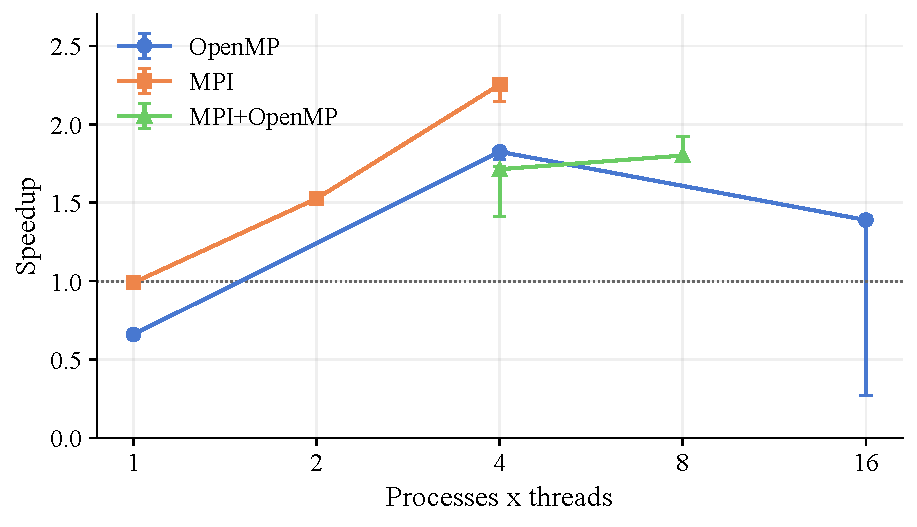
\includegraphics[width=0.90\linewidth]{figures/speedup_small.pdf}
    \caption{Ускорение на сетке $80\times80$. По горизонтали отложено произведение числа процессов и потоков; для гибрида $T_{\rm th}=4$. Маркеры показывают отношение медиан, отрезки показывают диапазон по повторам, определённый после формулы~\eqref{eq:speedup}. Пунктир соответствует $S=1$.}
    \label{fig:small-speedup}
\end{figure}

На обычной итерации программа выполняет четыре параллельные области OpenMP, а MPI-версия обменивается граничными слоями и вычисляет глобальные суммы.
Затраты на эти операции входят в измеренное время.
Их отдельный вклад на малой сетке не измерялся.

\FloatBarrier
\subsection{Крупные сетки}

Полные результаты приложения приведены в табл.~\ref{tab:large-omp}, \ref{tab:large-mpi} и~\ref{tab:large-hybrid}.
На сетке $400\times600$ все версии выполняют $1076$ итераций, на $800\times1200$ выполняют $2100$.
Последовательные базовые времена равны $3.473133$ и $28.095409$ с соответственно.

\begin{table}[H]
    \PaperTableStyle
    \begin{threeparttable}
        \caption{OpenMP на крупных сетках}
        \label{tab:large-omp}
        \begin{tabular*}{\linewidth}{@{\extracolsep{\fill}}rrrrr@{}}
            \toprule
            \textbf{Потоки} & \textbf{Итерации} & \textbf{$T$, с} & \textbf{Диапазон, с} & \textbf{$S$}\\
            \midrule
            \DataInput{large_omp_rows}
            \bottomrule
        \end{tabular*}
        \begin{tablenotes}[flushleft]\PaperTableNotesStyle
            \item[] Три повтора на одном узле. До 16 потоков используются отдельные физические ядра; 32 потока работают на 16 ядрах в режиме SMT2.
        \end{tablenotes}
    \end{threeparttable}
\end{table}

\begin{table}[H]
    \PaperTableStyle
    \begin{threeparttable}
        \caption{MPI на крупных сетках}
        \label{tab:large-mpi}
        \begin{tabular*}{\linewidth}{@{\extracolsep{\fill}}rrrrrr@{}}
            \toprule
            \textbf{Процессы} & \textbf{Итер.} & \textbf{Узлы} & \textbf{$T$, с} & \textbf{Диапазон, с} & \textbf{$S$}\\
            \midrule
            \DataInput{large_mpi_rows}
            \bottomrule
        \end{tabular*}
        \begin{tablenotes}[flushleft]\PaperTableNotesStyle
            \item[] Три повтора. Каждому процессу выделено отдельное физическое ядро. Конфигурация с 32 процессами использует по 16 ядер двух узлов.
        \end{tablenotes}
    \end{threeparttable}
\end{table}

\begin{table}[H]
    \PaperTableStyle
    \begin{threeparttable}
        \caption{MPI+OpenMP на крупных сетках}
        \label{tab:large-hybrid}
        \begin{tabular*}{\linewidth}{@{\extracolsep{\fill}}rrrrrrr@{}}
            \toprule
            \textbf{$P$} & \textbf{$T_{\rm th}$} & \textbf{Итер.} & \textbf{Узлы} & \textbf{$T$, с} & \textbf{Диапазон, с} & \textbf{$S$}\\
            \midrule
            \DataInput{large_hybrid_rows}
            \bottomrule
        \end{tabular*}
        \begin{tablenotes}[flushleft]\PaperTableNotesStyle
            \item[] Три повтора. Каждому потоку выделено отдельное физическое ядро; в конфигурации $4\times8$ по два процесса размещены на каждом из двух узлов.
        \end{tablenotes}
    \end{threeparttable}
\end{table}

На сетке $400\times600$ лучшие ускорения в проверенных конфигурациях равны $9.140$ для OpenMP, $13.995$ для MPI и $7.565$ для гибрида.
Эти значения получены при использовании 16 физических ядер одного узла.
На сетке $800\times1200$ наибольшее ускорение всей серии, $25.779$, даёт MPI с 32 процессами на двух узлах.
Гибрид $4\times8$ на тех же 32 физических ядрах достигает $S=15.933$.
OpenMP с 32 аппаратными потоками на 16 ядрах одного узла даёт $S=12.779$.
Одинаковое число программных исполнителей в этих трёх конфигурациях соответствует разным аппаратным ресурсам.

Ускорение MPI зависит от конфигурации немонотонно.
На сетке $400\times600$ переход от двух процессов к четырём увеличивает медиану времени с $1.772$ до $4.312$ с; при восьми процессах время снижается до $0.457$ с.
На сетке $800\times1200$ переход от восьми процессов к 16 увеличивает время с $3.521$ до $8.443$ с.
Эти замедления наблюдаются во всех трёх повторах (рис.~\ref{fig:large-speedup}).

\subsection{Границы интерпретации}

Измерения выполнены в одной сессии выделения ресурсов Polus с фиксированными компилятором и схемой размещения.
Диапазоны времени для крупных задач характеризуют разброс трёх повторов внутри этой сессии.
Время обменов, редукций и локальных операций отдельно не измерялось, поэтому причины немонотонных замедлений MPI не установлены.

В конфигурациях MPI с 32 процессами и гибрида $4\times8$ переход к двум узлам сопровождается увеличением числа физических ядер.
Сравнение одного и двух узлов при одинаковом числе ядер не проводилось, поэтому влияние межузлового размещения отдельно не оценено.

\begin{figure}[p]
    \centering
    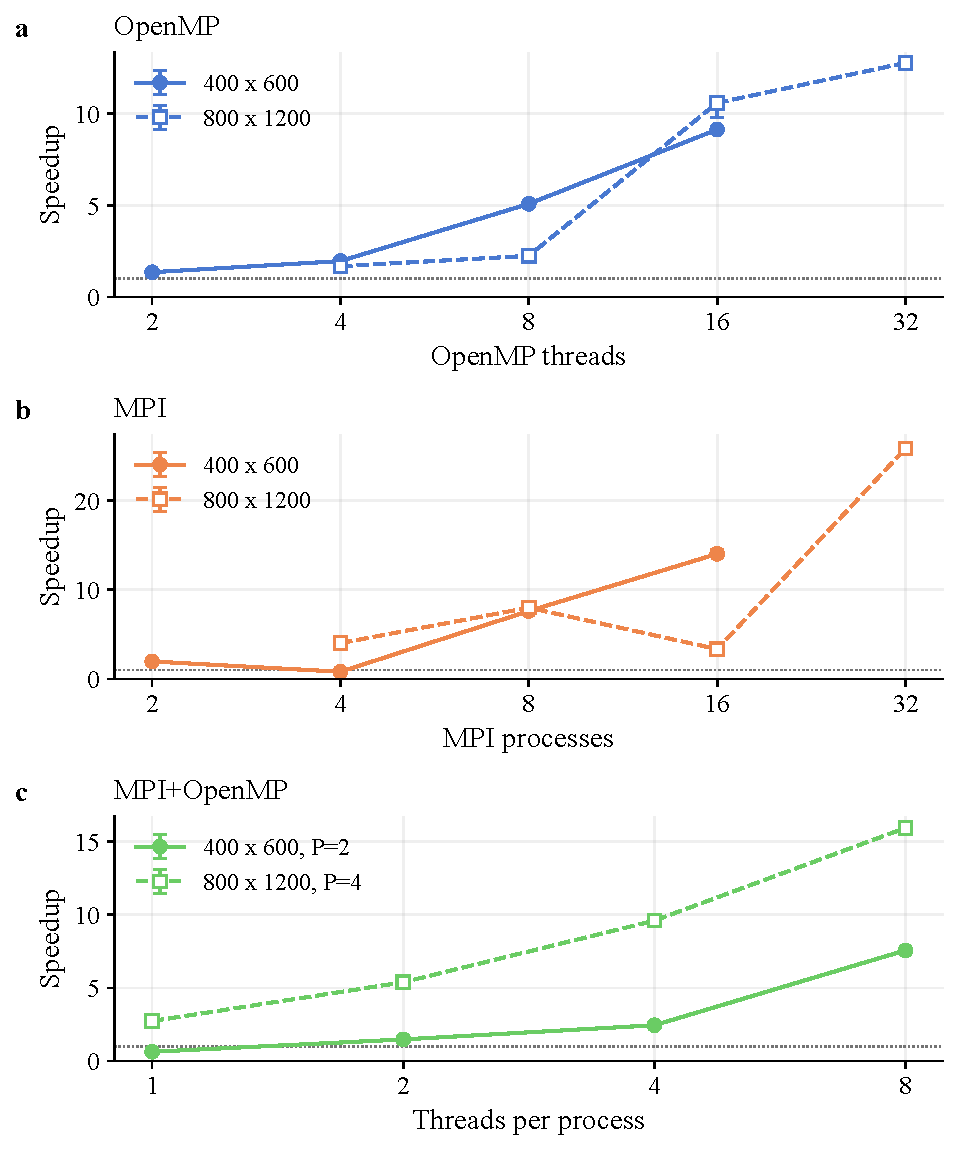
\includegraphics[width=\linewidth]{figures/speedup_large.pdf}
    \caption{Ускорение на крупных сетках: \textbf{a}
        OpenMP; \textbf{b} MPI; \textbf{c} MPI+OpenMP.
        Сплошная линия соответствует $400\times600$, штриховая линия соответствует $800\times1200$. Для гибрида число процессов фиксировано: $P=2$ на первой сетке и $P=4$ на второй. Отрезки показывают диапазон по повторам.
        OpenMP с 32 потоками использует SMT2 на одном узле; MPI с 32 процессами и гибрид $4\times8$ используют два узла.
    }
    \label{fig:large-speedup}
\end{figure}

\FloatBarrier
